\documentclass[a3,convert]{standalone}
\usepackage{pgfplots}
\usepgfplotslibrary{smithchart}    
\usepgfplotslibrary{polar}   
\usepackage{siunitx} 
\usepackage{tikz}
\pgfplotsset{compat=1.18}
\usetikzlibrary{calc,intersections,through}
\usepackage{comment}

\begin{document}

    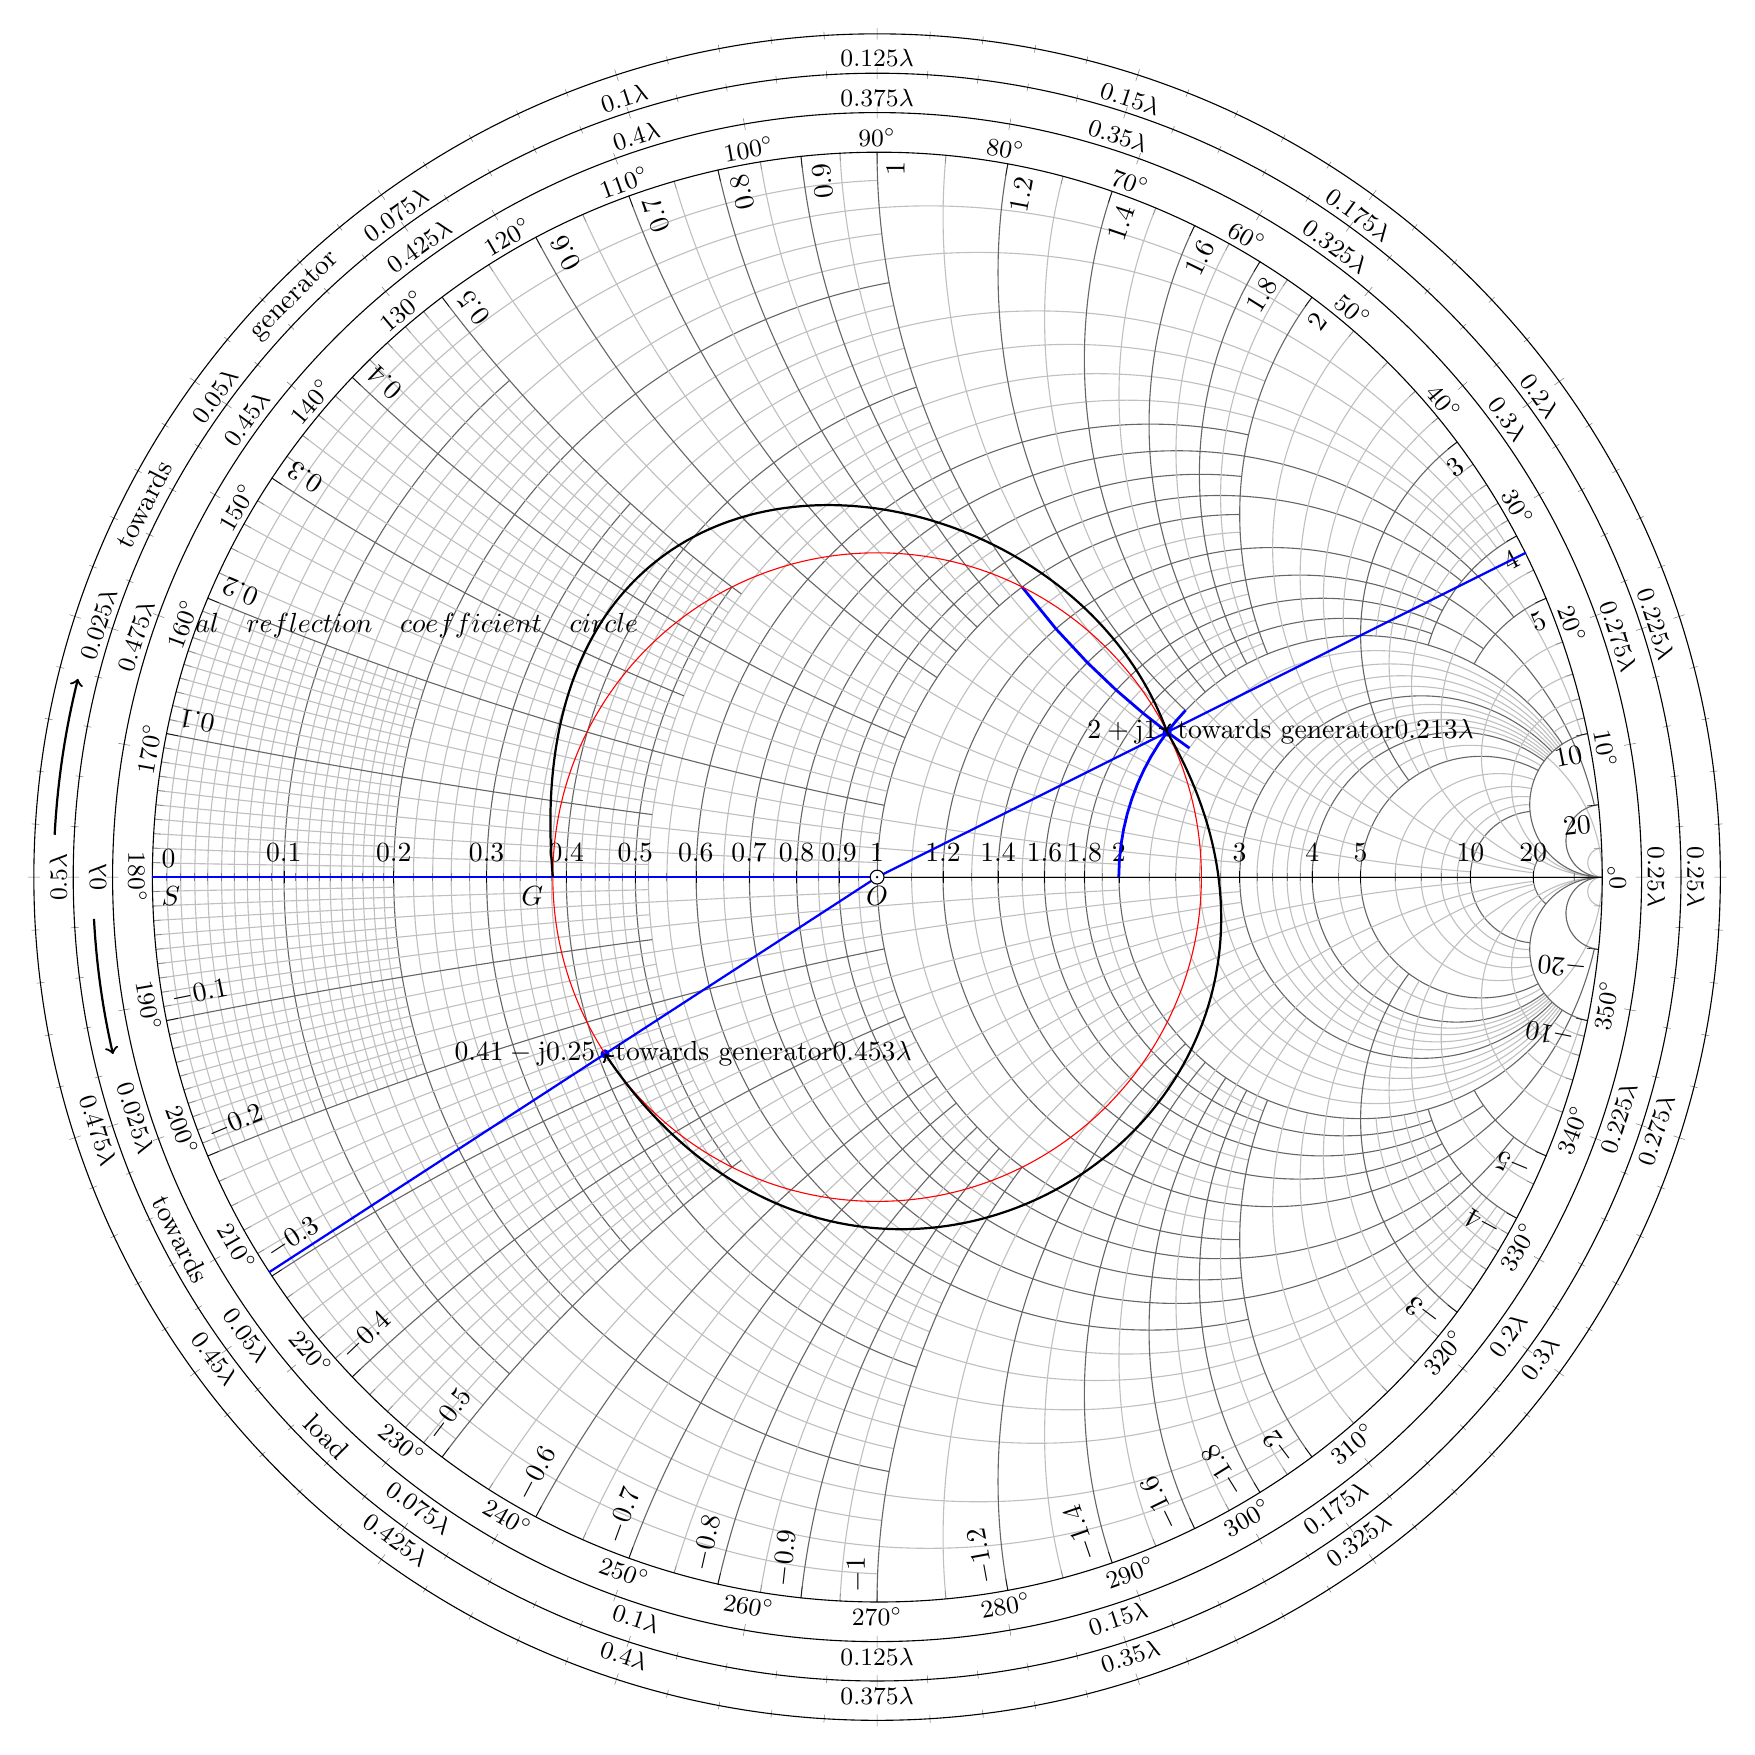
\begin{tikzpicture}
      \pgfmathsetmacro{\xoffset}{10.45*(1-cos(3))-1.25}  
      \pgfmathsetmacro{\yoffset}{sin(3)*10.45+9.2}  
      \draw[,thick,->] (+\xoffset,\yoffset) arc [radius=10.45cm,start angle=177,end angle=166];
      \pgfmathsetmacro{\xoffset}{10.45*(1-cos(18))-1.25}  
      \pgfmathsetmacro{\yoffset}{sin(18)*10.45+9.2} 
      \draw[,draw=none] (+\xoffset,\yoffset) arc [radius=10.45cm,start angle=162,end angle=144] node[midway,sloped]{towards};
      \pgfmathsetmacro{\xoffset}{10.45*(1-cos(36))-1.25}  
      \pgfmathsetmacro{\yoffset}{sin(36)*10.45+9.2} 
      \draw[,draw=none] (+\xoffset,\yoffset) arc [radius=10.45cm,start angle=144,end angle=126] node[midway,sloped]{generator};

      \pgfmathsetmacro{\xoffset}{9.95*(1-cos(-3))-0.75}  
      \pgfmathsetmacro{\yoffset}{sin(-3)*9.95+9.2} 
      \draw[,thick,->] (\xoffset,\yoffset) arc [radius=9.95cm,start angle=183,end angle=193] ;
      \pgfmathsetmacro{\xoffset}{9.95*(1-cos(-18))-0.75}  
      \pgfmathsetmacro{\yoffset}{sin(-18)*9.95+9.2} 
      \draw[,draw=none] (+\xoffset,\yoffset) arc [radius=10.45cm,start angle=198,end angle=216] node[midway,sloped]{towards};
      \pgfmathsetmacro{\xoffset}{9.95*(1-cos(-36))-0.75}  
      \pgfmathsetmacro{\yoffset}{sin(-36)*9.95+9.2} 
      \draw[,draw=none] (+\xoffset,\yoffset) arc [radius=10.45cm,start angle=216,end angle=234] node[midway,sloped]{load};


    \begin{polaraxis}[
                      rotate=180,
                      width=23cm,
                      xshift=1.5cm, 
                      yshift=1.5cm,
                      %xticklabels={$0\lambda$,$0.05\lambda$,$0.1\lambda$,$0.15\lambda$,$0.2\lambda$,$0.25\lambda$},
                      xticklabel style={
                          sloped like x axis={%
                              execute for upside down={\tikzset{anchor=south}},
                              reset nontranslations=false
                          },
                          anchor=north,
                      },
                      xticklabel={\small\pgfmathparse{0.5-\tick/720}\pgfmathprintnumber[fixed,precision=3]{\pgfmathresult}$\lambda$},
                      xtick align=center,
                      xtick={0,18,...,360},
                      grid=none,
                      axis y line = none,
                      minor x tick num={4},
                      ymax=1,
                     ]   
   \end{polaraxis}

    \begin{polaraxis}[
                      rotate=180,
                      width=22cm,
                      xshift=1cm, 
                      yshift=1cm,
                      %xticklabels={$0\lambda$,$0.05\lambda$,$0.1\lambda$,$0.15\lambda$,$0.2\lambda$,$0.25\lambda$},
                      xticklabel style={
                          sloped like x axis={%
                              execute for upside down={\tikzset{anchor=south}},
                              reset nontranslations=false
                          },
                          anchor=north,
                      },
                      xticklabel={\small\pgfmathparse{\tick/720}\pgfmathprintnumber[fixed,precision=3]{\pgfmathresult}$\lambda$},
                      xtick align=center,
                      xtick={0,18,...,360},
                      grid=none,
                      axis y line = none,
                      minor x tick num={4},
                      ymax=1,
                     ]    

    \end{polaraxis}



    \begin{polaraxis}[
                      width=21cm,
                      xshift=-0.5cm, 
                      yshift=-0.5cm,
                      %xticklabels={$0\lambda$,$0.05\lambda$,$0.1\lambda$,$0.15\lambda$,$0.2\lambda$,$0.25\lambda$},
                      xticklabel style={
                          sloped like x axis={%
                              execute for upside down={\tikzset{anchor=north}},
                              reset nontranslations=false
                          },
                          anchor=south,
                      },
                      xticklabel={\small\pgfmathprintnumber{\tick}\si{\degree}},
                      xtick align=center,
                      grid=none,
                      axis y line = none,
                     ]    
   \end{polaraxis}

   \begin{smithchart}[
                      show origin,
                      width=20cm,
                     ]
   
   \addplot[mark=none,line width=1,color=blue]
       coordinates{
           (2, 0) (2, 0.1) (2,0.2) (2,0.3) (2,0.4) (2,0.5) (2,0.6) (2,0.7) (2,0.8) (2,0.9) (2,1) (2,1.1) (2,1.2)
       };
   \addplot[mark=none,line width=1,color=blue]
       coordinates{
           (1, 1) (1.2, 1) (1.4,1) (1.6,1) (1.8,1) (2,1) (2.2,1) 
       };   
   %\addplot[mark=none,line width=0.5]
   %    coordinates{
   %        (1, 0) (-0.3, 0)  % this one is not drawn outside!!!
   %    };
      
       \coordinate [label=below:$O$] (a) at (1,0);
       \coordinate [label=330:$S$] (s) at (0,0);
       \coordinate [label=left:$2+\mathrm{j}1$] (b) at (2,1);    
       \path[draw=blue,fill=blue] (b) circle (0.05cm);
       \coordinate [label=left:$0.41-\mathrm{j}0.25$] (d) at (0.41,-0.25);
       \path [name path=S--A,draw=blue,thick] (s) -- (a);
       
       \path[draw=blue,fill=blue] (d) circle (0.05cm);
       \node (H) [label=135:$Equal\quad reflection\quad coefficient\quad circle$,name path=H,draw=red,circle through={(b)}] at (a) {};
       \path [name intersections={of=H and S--A,by={[label=210:$G$]G}}];

       \draw[thick,blue] (a) -- ($ (a) !2.3! (b) $) coordinate (c);
       \draw[thick,blue] (a) -- ($ (a) !2.3! (0.41,-0.25) $) coordinate (e);

       %%\draw[->,line width=2] (3,0) arc [start angle=0,end angle=120,radius=3]; 
       %%\draw [red,thick,domain=0:90] plot({2*cos(\x)},{2*sin(\x)});

       \draw[->,thick] (G) .. controls (0.1,0.5) and (0.6,1.3)  .. (b)node[anchor=west]{towards generator$0.213\lambda$};
       \draw[->,thick] (b) .. controls (2,-3.4) and (0.24,-0.95)  .. (0.41,-0.25)node[anchor=west]{towards generator$0.453\lambda$}; 
   

   \end{smithchart}

   \end{tikzpicture} 


\end{document}